\documentclass[11pt,a4paper]{article}

% ============================================================
% PACKAGES
% ============================================================

\usepackage[
    a4paper,
    left=2.0cm,
    right=2.0cm,
    top=1.55cm,
    bottom=1.55cm
]{geometry}

\usepackage[T1]{fontenc}
\usepackage{lmodern}
\usepackage{graphicx}
\usepackage{xcolor}
\usepackage{array}
\usepackage{tabularx}
\usepackage{ragged2e}
\usepackage{enumitem}
\usepackage{fancyhdr}
\usepackage{tikz}
\usetikzlibrary{positioning}
\usepackage{setspace}
\usepackage{needspace}

% ============================================================
% COLOUR
% ============================================================

\definecolor{TitleBlue}{RGB}{61,103,154}

% ============================================================
% GENERAL SETTINGS
% ============================================================

\setlength{\parindent}{0pt}
\setlength{\parskip}{0pt}
\renewcommand{\arraystretch}{1.0}

% ============================================================
% HEADINGS
% ============================================================

\newcommand{\blueheading}[1]{%
    {\sffamily\color{TitleBlue}\fontsize{15}{18}\selectfont #1}%
}

\newcommand{\bluebigheading}[1]{%
    {\sffamily\bfseries\color{TitleBlue}\fontsize{16}{19}\selectfont #1}%
}

% ============================================================
% ANSWER BOX
% ============================================================

\newcommand{\answerbox}[1]{%
    \vspace{2pt}
    \noindent
    \fbox{%
        \begin{minipage}[t]{%
            \dimexpr\textwidth-2\fboxsep-2\fboxrule\relax
        }
        \vspace{1mm}
        \itshape
        #1
        \vspace{1mm}
        \end{minipage}
    }
}

% ============================================================
% HEADER / FOOTER
% ============================================================

\pagestyle{fancy}
\fancyhf{}

\renewcommand{\headrulewidth}{0pt}
\renewcommand{\footrulewidth}{0pt}

\fancyhead[L]{%
    \sffamily\bfseries\itshape
    \fontsize{10.5}{12}\selectfont
    OPERATING SYSTEMS AND DATABASE MANAGEMENT SYSTEMS
}

\fancyhead[R]{%
    \sffamily\bfseries
    \fontsize{10.5}{12}\selectfont
    PROJECT PROPOSAL
}

\fancyfoot[R]{%
    \itshape
    \fontsize{10}{12}\selectfont
    Page \thepage
}

\setlength{\headheight}{14pt}
\setlength{\headsep}{23pt}
\setlength{\footskip}{24pt}

% ============================================================
% DOCUMENT
% ============================================================

\begin{document}

% ============================================================
% PAGE 1
% ============================================================

\vspace*{4mm}

\bluebigheading{PROJECT AND TEAM INFORMATION}

\vspace{13mm}

% ------------------------------------------------------------
% PROJECT TITLE
% ------------------------------------------------------------

\blueheading{Project Title}

\vspace{3mm}

\answerbox{
\textbf{Demonstrating Concurrent Railway Seat Allocation and Recommendation}
}

\vspace{13mm}

% ------------------------------------------------------------
% STUDENT / TEAM INFORMATION
% ------------------------------------------------------------

\blueheading{Student / Team Information}

\vspace{4mm}

\noindent
\begin{tabularx}{\textwidth}{
    |>{\RaggedRight\arraybackslash}p{0.52\textwidth}
    |>{\RaggedRight\arraybackslash}p{0.44\textwidth}|
}

% ============================================================
% TEAM NAME
% ============================================================

\hline

\begin{minipage}[t][0.8cm][t]{\linewidth}
\vspace{2mm}
\textit{Team Name:}
\end{minipage}
&
\begin{minipage}[t][0.8cm][t]{\linewidth}
\vspace{2mm}
\textit{Team Forge}
\end{minipage}

\\
\hline

% ============================================================
% MEMBER 1
% ============================================================

\begin{minipage}[t][4.2cm][t]{\linewidth}
\vspace{3mm}
\textbf{Team member 1 (Team Lead)}
\end{minipage}
&
\begin{minipage}[t][4.2cm][t]{\linewidth}
\vspace{2mm}

\textit{Kansal, Suryansh}\\
\textit{240211012}\\
\mbox{\textit{suryanshkansal123@gmail.com}}

\vspace{2mm}

\begin{center}
\includegraphics[
    width=2.7cm,
    height=1.85cm,
    keepaspectratio
]{suryanssh.jpeg}
\end{center}

\vfill

\end{minipage}

\\
\hline

% ============================================================
% MEMBER 2
% ============================================================

\begin{minipage}[t][4.2cm][t]{\linewidth}
\vspace{3mm}
\textbf{Team member 2}
\end{minipage}
&
\begin{minipage}[t][4.2cm][t]{\linewidth}
\vspace{2mm}

\textit{Dwivedi, Vidyansh}\\
\textit{24021654}\\
\mbox{\textit{dwivedividyansh@gmail.com}}

\vspace{2mm}

\begin{center}
\includegraphics[
    width=2.7cm,
    height=1.85cm,
    keepaspectratio
]{vidyansh.jpeg}
\end{center}

\vfill

\end{minipage}

\\
\hline

% ============================================================
% MEMBER 3
% ============================================================

\begin{minipage}[t][4.2cm][t]{\linewidth}
\vspace{3mm}
\textbf{Team member 3}
\end{minipage}
&
\begin{minipage}[t][4.2cm][t]{\linewidth}
\vspace{2mm}

\textit{Singh, Arjun}\\
\textit{24021107}\\
\mbox{\textit{arjunsinghgodara@gmail.com}}

\vspace{2mm}

\begin{center}
\includegraphics[
    width=2.7cm,
    height=1.85cm,
    keepaspectratio
]{arjun.jpeg}
\end{center}

\vfill

\end{minipage}

\\
\hline

\end{tabularx}

\newpage

% ============================================================
% PAGE 2
% ============================================================

\bluebigheading{PROPOSAL DESCRIPTION (10 pts)}

\vspace{9mm}

% ============================================================
% MOTIVATION
% ============================================================

\blueheading{Motivation (1 pt)}

\vspace{3mm}

\answerbox{
Railway reservation is a good example of a system where many users may request the same resource at the same time.For example, two passengers may try to book the same seat at the same time or request goes at same time. If the requests are not handled properly,the same seat could be given to both passengers or the available seat count could become wrong .

In this project, we want to build a railway reservation system that helps us understand how Operating System and DBMS concepts work together. The system will keep details of trains, seats, passengers, and bookings in a database.

We will also create a test where several users try to book seats at the same time. This will help us see problems such as race conditions and then solve them using threads,synchronization,locks and database transactions.

Another part of our project is a train recommendation feature.A passenger can decide what is more important to them, such as a cheaper ticket, shorter travel time, more available seats, or departure time.The system will use these choices to rank the available trains.
}

\vspace{7mm}

% ============================================================
% STATE OF THE ART
% ============================================================

\blueheading{State of the Art / Current solution (1 pt)}

\vspace{3mm}

\answerbox{
Railway booking systems already provide features such as train search, seat availability, and ticket booking.They store information about trains, passengers,seats,and bookings in databases.Since many users can use the system at the same time,the database has to handle these requests without causing incorrect bookings.

Most train search systems provide filters such as price, timing, route, and journey duration. In our project,we are adding a simple personalized recommendation feature along with these normal search options.

The user will be able to give more importance to the things they care about. For example, someone who wants to spend less money can give a higher priority to price.Someone else may prefer a shorter journey. The system will use these priorities to calculate scores and suggest the suitable trains accordingly.
}

\vspace{7mm}

% ============================================================
% PROJECT GOALS AND MILESTONES
% ============================================================

\needspace{10cm}

\blueheading{Project Goals and Milestones (2 pts)}

\vspace{3mm}

\answerbox{
The main goal of our project is to make a railway reservation system that can handle multiple booking requests correctly. We also want to use the project to practically demonstrate the OS and DBMS concepts that we have studied.

The main steps of the project are:

\begin{enumerate}[leftmargin=*,nosep]

    \item Create database tables for trains, seats, passengers, and bookings.

    \item Add basic features such as train search, checking available seats, booking and cancellation.

    \item Add the personalized train recommendation feature.

    \item Allow the passenger to give an importance value from 1 to 5 for price,journey duration,seat availability and departure time.

    \item Convert the different train details into scores between 0 and 100.

    \item Calculate the final weighted score for every train that satisfies the passenger's basic requirements.

    \item Arrange the trains according to their final scores and display the better options first.

    \item Use multiple threads to represent passengers trying to book seats at the same time.

    \item Demonstrate the race condition that can happen when multiple requests try to access the same seat.

    \item Use synchronization and locking to make sure that a seat cannot be successfully booked by two passengers.

    \item Use database transactions with COMMIT and ROLLBACK while processing bookings.

    \item Use database isolation and constraints to maintain correct booking information.

    \item Create a controlled deadlock situation and show how it can be detected and handled.

    \item Build an interface through which the booking, seat availability, and recommendation results can be viewed.

\end{enumerate}
}

\vspace{8mm}

% ============================================================
% PAGE 3
% ============================================================

% ============================================================
% PROJECT APPROACH
% ============================================================

\blueheading{Project Approach (3 pts)}

\vspace{4mm}

\answerbox{
The project will have three main parts:user interface,the backend that handles the railway operations and the database.

The database will store information about trains, seats, passengers, and bookings.Each seat will be connected to a particular train so that its status can be maintained separately.

When a passenger searches for a train,the system will first check the basic requirements such as source,destination, journey date, and maximum budget. Trains that do not match these requirements will not be considered for recommendation they will get filtered out.

After this filtering,the remaining trains will be compared using four factors:price, journey duration, seat availability, and departure time. Each factor will be converted into a score between 0 and 100.A cheaper train will get a better price score,while a shorter journey will get a better duration score. A train with more available seats will get a higher availability score.The departure-time score will depend on how close the train is to the time preferred by the passenger.

The passenger will give an importance value from 1 to 5 for each factor. These values will be converted into weights and used to calculate the final score of every eligible train.The trains will then be sorted using these scores.

For booking,the passenger will select a train and seat.To demonstrate concurrency,multiple threads will be made to send booking requests at the same time.Synchronization and database transactions will be used so that two passengers cannot successfully reserve the same seat.

We will also create a few test case where two transactions wait for resources held by each other. This will demonstrate how a deadlock can occur and how it can be detected and handled.

Java will be used for the backend and multithreading.MySQL or PostgreSQL will be used as the database, while HTML, CSS, and JavaScript will be used for the interface.
}

\vspace{7mm}

\newpage
% ============================================================
% SYSTEM ARCHITECTURE
% ============================================================

\blueheading{System Architecture (High Level Diagram)(2 pts)}

\vspace{5mm}

\begin{center}

\begin{tikzpicture}[
    node distance=7mm and 12mm,
    box/.style={
        draw,
        rounded corners,
        align=center,
        minimum width=5.0cm,
        minimum height=0.85cm,
        font=\small
    },
    smallbox/.style={
        draw,
        rounded corners,
        align=center,
        minimum width=4.3cm,
        minimum height=1.05cm,
        font=\small
    },
    arrow/.style={
        ->,
        thick
    }
]

\node[box] (ui) {
    User Interface\\
    Search / Preferences / Booking / Simulation
};

\node[box, below=of ui] (recommendation) {
    Personalized Train Recommendation\\
    Filtering / Scoring / Ranking
};

\node[box, below=of recommendation] (backend) {
    Railway Allocation Engine\\
    Concurrent Request Processing
};

\node[smallbox, below left=of backend] (os) {
    Operating System\\
    Threads / Synchronization\\
    Locks / Deadlock
};

\node[smallbox, below right=of backend] (dbms) {
    DBMS\\
    Transactions / ACID\\
    Isolation / Constraints
};

\node[box, below=19mm of backend] (database) {
    Railway Database\\
    TRAIN \quad SEAT \quad PASSENGER \quad BOOKING
};

\draw[arrow] (ui) -- (recommendation);

\draw[arrow] (recommendation) -- (backend);

\draw[arrow] (backend) -- (os);

\draw[arrow] (backend) -- (dbms);

\draw[arrow] (os) -- (database);

\draw[arrow] (dbms) -- (database);

\end{tikzpicture}

\end{center}

\vspace{5mm}

% ============================================================
% PROJECT OUTCOME
% ============================================================

\needspace{7cm}

\blueheading{Project Outcome / Deliverables (1 pts)}

\vspace{3mm}

\answerbox{
The final result will be a working railway reservation system with train search,seat checking,booking,cancellation and personalized train recommendations.

For the recommendation feature,the system will show the scores used to rank the trains.This will make it possible to see why one train was placed above another instead of only showing the final result.

The booking part will include a concurrency demonstration.Several threads will try to make bookings at the same time. This will allow us to show what happens during a race condition and how synchronization and database transactions can prevent incorrect seat allocation.

The project will also include a deadlock demonstration.Along with the application, we will prepare the database tables, SQL scripts, recommendation logic,test cases,concurrency tests, and project documentation.
}

\vspace{7mm}

% ============================================================
% ASSUMPTIONS
% ============================================================

\blueheading{Assumptions}

\vspace{3mm}

\answerbox{
The project will use a fixed set of railway data instead of live railway data.Trains will have predefined routes,timings,fares and seats.

Source,destination,journey date,and maximum budget will be treated as the basic requirements for searching. Price, journey duration, seat availability, and departure time will be used for the recommendation.

The importance value for each recommendation factor will be between 1 and 5. The initial demonstration may use one route and a limited number of seats, but the database structure will be able to support multiple trains.

Payment processing,live railway booking, and other real-world railway services are outside the scope of this project.
}

% ============================================================
% PAGE 4 - REFERENCES
% ============================================================

\clearpage

\blueheading{References}

\vspace{6mm}

\answerbox{
\begin{enumerate}[leftmargin=*,itemsep=3mm]

    \item Abraham Silberschatz, Peter B. Galvin, Greg Gagne,
    \textit{Operating System Concepts}.

    \item Abraham Silberschatz, Henry F. Korth, S. Sudarshan,
    \textit{Database System Concepts}.

    \item Oracle Java Documentation -- Threads and Concurrency.

    \item MySQL Documentation -- Transactions, Locking, and
    Isolation Levels.

    \item PostgreSQL Documentation -- Transactions and
    Concurrency Control.

\end{enumerate}
}

\end{document}